\cleardoublepage
\chapter{Results}
\label{ch:results}
\label{ch:chapter4}

\section{Retrieval Results}

\subsection{Baselines}

We first evaluated the retrieval performance of our baseline systems introduced in Section \ref{baselines_sec}. We found that ColBERTv2 consistently demonstrated strong performance across all datasets. In contrast, HippoRAG showed particularly high retrieval performance on MuSiQue, which is attributed to the dataset’s entity-centric design \cite{NEURIPS2024_6ddc001d}. However, HippoRAG underperformed on easier datasets relative to simpler methods like BM25. 

\noindent We also observe that MuSiQue and 2Wiki have the lowest overall retrieval scores. This is consistent with the design of these benchmarks, which introduce complexity through actual multi-hop reasoning.

\noindent Table \ref{tab:retrieval_results} and Table \ref{tab:avg_retrieval_results} summarize retrieval performance across all baseline systems, reporting \textbf{recall@k} for various values of $k$. Importantly, the vast majority of questions in the datasets require no more than five passages as supporting evidence, which highlights the importance of high recall at low values of $k$ to reduce irrelevant content during the question answering phase.

\begin{table}[ht]
    \centering
    \setlength{\tabcolsep}{2pt}
    \resizebox{\textwidth}{!}{
        \begin{tabular}{lcccccccccccccccccccc}
            \toprule
            & \multicolumn{5}{c}{\textbf{LoCoMo}} & \multicolumn{5}{c}{\textbf{HotpotQA}} & \multicolumn{5}{c}{\textbf{2Wiki}} & \multicolumn{5}{c}{\textbf{MuSiQue}}\\
            \cmidrule(lr){2-6} \cmidrule(lr){7-11} \cmidrule(lr){12-16} \cmidrule(lr){17-21}
             $k$ & 2 & 5 & 10 & 20 & 100 & 2 & 5 & 10 & 20 & 100 & 2 & 5 & 10 & 20 & 100 & 2 & 5 & 10 & 20 & 100 \\
            \midrule
            BM25 & 41.6 & 52.7 & 60.3 & 66.3 & 78.6 & 50.7 & 63.6 & 74.6 & 
83.1 & \underline{91.2} & 45.6 & 57.2 & 62.8 & 66.4 & 72.7 & 29.2 & 38.3 & 45.1 & 50.8 & 64.7 \\
            msmarco-bert-base-dot-v5 & \underline{42.5} & \underline{54.5} & \underline{62.2} & \underline{70.0} & \underline{86.0} & \underline{56.2} & 67.0 & 72.5 & 76.8 & 84.8 & \textbf{54.3} & \underline{62.7} & \underline{66.0} & \underline{68.4} & 73.0 & \underline{36.5} & \underline{46.4} & \underline{54.0} & \underline{60.6} & \underline{73.7} \\
            ColBERTv2 & \textbf{54.8} & \textbf{66.6} & \textbf{73.5} & \textbf{80.0} & \textbf{89.6} & \textbf{61.8} & \textbf{74.8} & \textbf{81.0} & \textbf{85.3} & \underline{91.2} & \underline{53.6} & \textbf{62.8} & \textbf{67.1} & \textbf{69.9} & \underline{74.5} & 35.1 & 45.4 & 52.1 & 57.7 & 71.4 \\
            \midrule
            HippoRAG (QWen2.5-14B) & - & - & - & - & - & 53.4 & 67.8 & 75.5 & 80.5 & 88.5 & 39.6 & 48.3 & 54.0 & 59.0 & 68.2 & 35.2 & 46.1 & 53.6 & 60.1 & 72.7 \\
            HippoRAG (GPT-4o-mini) & - & - & - & - & - & \underline{58.4} & \underline{73.3} & \underline{80.3} & \underline{84.7} & \textbf{91.5} & 51.0 & 59.8 & 64.1 & 68.1 & \textbf{75.3} & \textbf{38.4} & \textbf{50.2} & \textbf{58.1} & \textbf{64.7} & \textbf{76.4} \\
            \bottomrule
            \multicolumn{21}{p{18cm}}{\rule{0pt}{3ex} \textbf{Bold} values indicate the best score, while \underline{underlined} values indicate the second-best score.} \\
        \end{tabular}
     }
    \caption{Recall@$k$ performance of RAG systems: ColBERTv2, msmarco-bert-base-dot-v5, BM25, and HippoRAG.}
    \label{tab:retrieval_results}
\end{table}
\begin{table}[ht]
    \centering
    \begin{tabular}{lccccc}
            \toprule
            & \multicolumn{5}{c}{\textbf{Average}} \\
            \cmidrule(lr){2-6}
             K & \small 2 & \small 5 & \small 10 & \small 20 & \small 100 \\
            \midrule
            \small BM25 & 41.8 & 53.0 & 60.8 & 66.8 & 76.2 \\
            \small msmarco-bert &
49.0 & 58.7 & 64.2 & 68.6 & 77.2 \\
            \small ColBERTv2 & \textbf{50.2} & \underline{61.0} & \underline{66.7} & \underline{71.0} & \underline{79.0} \\
            \midrule
            \small HippoRAG (Qwen2.5-14B) & 42.7 & 54.1 & 61.0 & 66.5 & 76.5 \\
            \small HippoRAG (GPT-4o-mini) &  \underline{49.3} & \textbf{61.1} & \textbf{67.5} & \textbf{72.5} & \textbf{81.1} \\
            \bottomrule
        \end{tabular}
    \caption{Average baselines retrieval performance on MHQA datasets (HotpotQA, 2Wiki, MuSiQue).}
    \label{tab:avg_retrieval_results}
\end{table}

\subsection{Cognitive Language Agents}

\noindent We evaluated the retrieval performance of the language agent architectures introduced in Section \ref{agents_sec}. Unlike static retrieval baselines, these agents typically execute multiple searches while reasoning about a question, rather than issuing a single query. Consequently, the retrieved results form an unranked set of documents, and we evaluate performance using macro recall (R), macro precision (P), and macro $F_1$. 

\noindent We start with experimenting with the strongest retrievers, ColBERTv2 and HippoRAG, for the QA Agent. We found that the agent achieved similar retrieval performance with both. Results are shown in Table \ref{tab:retrieval_results_qa_agent}.

\begin{table}[ht]
    \centering
    \adjustbox{max width=\textwidth}{
        \begin{tabular}{lcccccccccccccccccc}
            \toprule
            & \multicolumn{3}{c}{\textbf{HotpotQA}} & \multicolumn{3}{c}{\textbf{2Wiki}} & \multicolumn{3}{c}{\textbf{MuSiQue}} & \multicolumn{3}{c}{ \textbf{Average}} \\
            \cmidrule(lr){2-4} \cmidrule(lr){5-7} \cmidrule(lr){8-10} \cmidrule(lr){11-13}
             & R & P & $F_1$ & R & P & $F_1$ & R & P & $F_1$ & R & P & $F_1$ \\
            \midrule
            \scriptsize QA Agent (ColBERTv2) & 85.8 & 23.9 & 36.6 & 90.3 & 21.6 & 34.4 & 69.0 & 17.7 & 27.5 & 81.7 & 21.1 & 32.8 \\
             \scriptsize QA Agent (HippoRAG) & 84.6 & 24.3 & 37.0 & 90.2 & 22.4 & 35.3 & 70.6 & 18.9 & 29.2 & 81.8 & 21.9 & 33.8 \\
            \bottomrule
        \end{tabular}
    }
    \caption{QA Agent retrieval performance with both ColBERTv2 and HippoRAG on MHQA datasets.}
    \label{tab:retrieval_results_qa_agent}
\end{table}

\noindent Considering that we did not observe any significant difference between our two retrievers, we only tested ColBERTv2 on each of the QA Agent variants shown in Table \ref{tab:retrieval_results_qa_variants}.

\begin{table}[ht]
    \centering
    \adjustbox{max width=\textwidth}{
        \begin{tabular}{lcccccccccccccccccc}
            \toprule
             & \multicolumn{3}{c}{\textbf{HotpotQA}} & \multicolumn{3}{c}{\textbf{2Wiki}} & \multicolumn{3}{c}{\textbf{MuSiQue}} & \multicolumn{3}{c}{ \textbf{Average}} \\
            \cmidrule(lr){2-4} \cmidrule(lr){5-7} \cmidrule(lr){8-10} \cmidrule(lr){11-13}
             & R & P & $F_1$ & R & P & $F_1$ & R & P & $F_1$ & R & P & $F_1$ \\
            \midrule
            Re-Ranking & 82.3 & 61.3 & 65.2 & 87.5 & 73.6 & 76.9 & 62.8 & 49.2 & 51.0 & 77.5 & 61.4 & 64.4 \\
            Pagination & 86.1 & 23.2 & 35.6 & 91.7 & 20.2 & 32.4 & 69.0 & 16.5 & 25.9 & 82.3 & 18.8 & 31.3 \\
            Self-Reflection & 85.1 & 24.1 & 36.8 & 89.5 & 21.8 & 34.5 & 68.6 & 18.0 & 27.9 & 81.1 & 21.3 & 33.1 \\
            \bottomrule
        \end{tabular}
    }
    \caption{Retrieval performance of QA Agent variants with ColBERTv2 and GPT-4o-mini on MHQA datasets, measured using Recall (R), Precision (P), and $F_1$.}
    \label{tab:retrieval_results_qa_variants}
\end{table}

\noindent The QA Agent with Re-ranking shows a modest drop in recall relative to the base agent, but its precision improves substantially. This indicates that the second-stage LLM-based retriever effectively prunes distractors, resulting in fewer irrelevant passages to reason over.

\noindent The QA Agent with Pagination exhibits slight improvements in recall across datasets, though the gains are smaller than anticipated. We hypothesize that this is due to inherent limitations of the retriever. In particular, Weller et al.  show empirically that multi-vector retrievers such as ColBERTv2 can only represent a restricted set of top-$k$ rankings, limiting the benefit of retrieving beyond the initial candidate set \cite{weller2025theoreticallimitationsembeddingbasedretrieval}.

\noindent We now compare the strongest QA Agent variant that implements reflection with the QA DAG Agent in Table \ref{tab:retrieval_results_agents}.

\begin{table}[ht]
    \centering
    \adjustbox{max width=\textwidth}{
        \begin{tabular}{lccccccccccccccccccccc}
            \toprule
            & \multicolumn{3}{c}{\scriptsize \textbf{LoCoMo}} & \multicolumn{3}{c}{\scriptsize \textbf{HotpotQA}} & \multicolumn{3}{c}{\scriptsize \textbf{2Wiki}} & \multicolumn{3}{c}{\scriptsize \textbf{MuSiQue}} & \multicolumn{3}{c}{\scriptsize \textbf{Average}} \\
            \cmidrule(lr){2-4} \cmidrule(lr){5-7} \cmidrule(lr){8-10} \cmidrule(lr){11-13} \cmidrule(lr){14-16}
             & \scriptsize R & \scriptsize P & \scriptsize $F_1$ & \scriptsize R & \scriptsize P & \scriptsize $F_1$ & \scriptsize R & \scriptsize P & \scriptsize $F_1$ & \scriptsize R & \scriptsize P & \scriptsize $F_1$ & \scriptsize R & \scriptsize P & \scriptsize $F_1$ \\
             \midrule
            \scriptsize QA Agent & 62.1 & 15.4 & 23.7 & 85.8 & 23.9 & 36.6 & 90.3 & 21.6 & 34.4 & 69.0 & 17.7 & 27.5 & 76.8 & 19.7 & 30.6 \\
            \scriptsize Re-Ranking Agent & - & - & - & - & - & - & - & - & - & - & - & - & - & - & - \\
            \scriptsize Hybrid QA Agent & - & - & - & - & - & - & - & - & - & - & - & - & - & - & - \\
            \scriptsize Multi-agent Reflection & - & - & - & - & - & - & - & - & - & - & - & - & - & - & - \\
            \bottomrule
        \end{tabular}
    }
    \caption{\small Agents Retrieval performance.}
    \label{tab:retrieval_results_agents}
\end{table}

\noindent Overall, even the simplest agent, the QA Agent, substantially outperforms all baselines on 2Wiki and MuSiQue. On MuSiQue, the QA Agent retrieves an average of $10.9$ unique documents per query, achieving a recall of $69.0$, compared to $60.6$ for ColBERTv2 at $k = 20$. On 2Wiki, the QA Agent retrieves $10.4$ unique documents on average and achieves a recall of $90.3$, representing a $15.8$ point improvement over msmarco-bert-base-dot-v5 at $k = 100$. In contrast, on LoCoMo, the QA Agent performs slightly worse, even when compared against $R@5$. 


\section{Question Answering Results}

\subsection{Baselines}

\noindent Figure \ref{fig:scores_gpt4o} shows the results obtained using GPT-4o-mini across the four datasets using ColBERTV2, msmarco-bert-base-dot-v5, and BM25 retrievers. While performance generally improves with increasing $k$, the gains diminish as more irrelevant details begin to interfere with the model's ability to identify relevant information within its context.

\noindent Interestingly, a performance drop is observed on LoCoMo, HotpotQA, and 2Wiki under the FULL-CONTEXT setup, which suggests that excessive context introduces noise. However, MuSiQue, the most complex dataset, benefits modestly from the added information.

\begin{figure}[!h]
\centering

\begin{subfigure}[b]{1.0\textwidth}
    \input{chapter4/scoresgpt4o/score_context}
    \vspace{-1.5em}
    \caption{ColBERTv2}\label{fig:scores_colbert}
\end{subfigure}

\vspace{0.5em}

\begin{subfigure}[b]{0.48\textwidth}
    \input{chapter4/scoresgpt4o/score_context_dense}
    \caption{msmarco-bert-base-dot-v5}\label{fig:scores_dense}
\end{subfigure}
\begin{subfigure}[b]{0.48\textwidth}
    \input{chapter4/scoresgpt4o/score_context_bm25}
    \caption{BM25}\label{fig:scores_bm25}
\end{subfigure}

\caption{QA performance of RAG systems with GPT-4o-mini: (a) ColBERTv2, (b) msmarco-bert-base-dot-v5, and (c) BM25, measured using Exact Match (EM), ROUGE-1 ($R_1$), ROUGE-2 ($R_2$), and an LLM-based score ($L_1$).}
\label{fig:scores_gpt4o}
\end{figure}

\noindent We also evaluate Qwen2.5-14B using a slightly adapted prompt, see Appendix \ref{fig:qa-base-qwen}.  As shown in Figure \ref{fig:scores_qwen}, its performance closely matches that of GPT-4o-mini, demonstrating that smaller models with strong instruction tuning can achieve competitive results.

\begin{figure}[!h]
\centering

\begin{subfigure}[b]{1.0\textwidth}
    \input{chapter4/scoresqwen/score_context}
    \vspace{-1.5em}
    \caption{ColBERTv2}\label{fig:scores_colbert_qwen}
\end{subfigure}

\vspace{0.5em}

\begin{subfigure}[b]{0.48\textwidth}
    \input{chapter4/scoresqwen/score_context_dense}
    \caption{msmarco-bert-base-dot-v5}\label{fig:scores_dense_qwen}
\end{subfigure}
\begin{subfigure}[b]{0.48\textwidth}
    \input{chapter4/scoresqwen/socre_context_bm25}
    \caption{BM25}\label{fig:scores_bm25_qwen}
\end{subfigure}

\caption{QA performance of RAG systems with Qwen2.5-14B-Instruct: (a) ColBERTv2, (b) msmarco-bert-base-dot-v5, and (c) BM25, measured using Exact Match (EM), ROUGE-1 ($R_1$), ROUGE-2 ($R_2$), and an LLM-based score ($L_1$).}
\label{fig:scores_qwen}
\end{figure}

\noindent We also test o3-mini using $k = 5$. As expected, o3-mini matches or outperforms other models with higher $k$ values, suggesting that reasoning ability plays a key role for MHQA task.

\noindent For reference, we include results when only relevant documents are provided to the LLM directly in Table \ref{tab:qa_results_default}, and results when all the corpus is passed to the LLM in Table \ref{tab:qa_results_fullcontext}.

\begin{table}[ht]
    \centering
        \setlength{\tabcolsep}{3pt}
        \adjustbox{max width=\textwidth}{
        \begin{tabular}{lcccccccccccccccccccc}
            \toprule
            & \multicolumn{4}{c}{\textbf{LoCoMo}} & \multicolumn{4}{c}{\textbf{HotpotQA}} & \multicolumn{4}{c}{\textbf{2Wiki}} & \multicolumn{4}{c}{\textbf{MuSiQue}} & \multicolumn{4}{c}{\textbf{Average}} \\
            \cmidrule(lr){2-5} \cmidrule(lr){6-9} \cmidrule(lr){10-13} \cmidrule(lr){14-17} \cmidrule(lr){18-21}
             & EM & $R_1$ & $R_2$ & $L_1$ & EM & $R_1$ & $R_2$ & $L_1$ & EM & $R_1$ & $R_2$ & $L_1$ & EM & $R_1$ & $R_2$ & $L_1$ & EM & $R_1$ & $R_2$ & $L_1$ \\
            \midrule
            GPT-4o-mini & 36.0 & 66.1 & 37.5 & 62.0 & 63.7 & 77.2 & 43.6 & 78.0 & 56.9 & 64.2 & 43.6 & 63.0 & 46.5 & 54.8 & 37.5 & 52.0 & 50.1 & 65.6 & 40.6 & 63.8 \\
            o3-mini & 33.8 & 65.5 & 37.2 & 69.0 & 68.0 & 83.1 & 48.5 & 85.0 & 68.3 & 77.1 & 54.1 & 77.0 & 65.9 & 76.7 & 56.1 & 76.0 & 59.0 & 75.6 & 49.0 & 76.8 \\
            Qwen2.5-14B & 35.0 & 63.3 & 35.0 & 58.0 & 59.0 & 72.9 & 44.1 & 75.0 & 57.3 & 65.6 & 47.1 & 65.0 & 38.3 & 45.7 & 32.2 & 44.0 & 47.4 & 61.9 & 39.6 & 60.5 \\
            \bottomrule
        \end{tabular}
        }
    \caption{Question Answering performance when only the supporting passages are provide to the model.}
    \label{tab:qa_results_default}
\end{table}

\begin{table}[!h]
    \centering
        \setlength{\tabcolsep}{3pt}
        \resizebox{\textwidth}{!}{
        \begin{tabular}{cccccccccccccccccccc}
            \toprule
            \multicolumn{4}{c}{\textbf{LoCoMo}} & \multicolumn{4}{c}{\textbf{HotpotQA}} & \multicolumn{4}{c}{\textbf{2Wiki}} & \multicolumn{4}{c}{\textbf{MuSiQue}} \\
            \cmidrule(lr){1-4} \cmidrule(lr){5-8} \cmidrule(lr){9-12} \cmidrule(lr){13-16}
             EM & $R_1$ & $R_2$ & $L_1$ & EM & $R_1$ & $R_2$ & $L_1$ & EM & $R_1$ & $R_2$ & $L_1$ & EM & $R_1$ & $R_2$ & $L_1$ \\
            \midrule
            16.7 & 40.6 & 21.8 & 43.0 & 42.0 & 54.1 & 29.7 & 54.3 & 30.0 & 35.0 & 22.5 & 33.0 & 19.5 & 29.7 & 15.2 & 23.0 \\
            \bottomrule
        \end{tabular}
        }
    \caption{QA performance of the FULL-CONTEXT setup with GPT-4o-mini ($128k$ tokens), measured using Exact Match (EM), ROUGE-1 ($R_1$), ROUGE-2 ($R_2$), and an LLM-based score ($L_1$).}
    \label{tab:qa_results_fullcontext}
\end{table}

\noindent Detailed results for baseline configurations that use simple retrieval methods are provided in Table \ref{tab:qa_results}.

\input{chapter4/qa_results}

\noindent Finally, we include QA results from HippoRAG \cite{NEURIPS2024_6ddc001d} in Table \ref{tab:qa_hippo_rag_results}, which incorporates graph-structured memory. HippoRAG performs especially well on the MuSiQue dataset, likely due to its ability to abstract relationships and reason over structured content.

\begin{table}[ht]
    \centering
        \setlength{\tabcolsep}{3pt}
        \resizebox{\textwidth}{!}{
        \begin{tabular}{lcccccccccccccccccccc}
            \toprule & \multicolumn{4}{c}{\textbf{HotpotQA}} & \multicolumn{4}{c}{\textbf{2Wiki}} & \multicolumn{4}{c}{\textbf{MuSiQue}} & \multicolumn{4}{c}{\textbf{Average}} \\
            \cmidrule(lr){2-5} \cmidrule(lr){6-9} \cmidrule(lr){10-13} \cmidrule(lr){14-17}
             & EM & $R_1$ & $R_2$ & $L_1$ & EM & $R_1$ & $R_2$ & $L_1$ & EM & $R_1$ & $R_2$ & $L_1$ & EM & $R_1$ & $R_2$ & $L_1$ \\
            \midrule
            HippoRAG (QWen2.5-14B) & 34.3 & 48.0 & 25.7 & 53.0 & 14.7 & 23.0 & 12.5 & 23.0 & 12.5 & 20.2 & 11.9 & 19.0 & 20.5 & 30.4 & 16.7 & 31.7 \\
            HippoRAG (GPT-4o-mini) & 46.0 & 61.0 & 34.4 & - & - & - & - & - & 25.3 & 36.7 & 22.8 & 34.0 & - & - & - & - \\
            \bottomrule
        \end{tabular}
        }
    \caption{\small HippoRAG Question Answering performance with both QWen2.5-14B and GPT-4o-mini using Contriever as the embedding model.}
    \label{tab:qa_hippo_rag_results}
\end{table}

\subsection{Cognitive Language Agents}

\noindent Table \ref{tab:qa_results_agent} reports the QA performance of the agent architectures. Even the simplest variant, the QA Agent, significantly outperforms the baseline methods on HotpotQA, 2Wiki, and MuSiQue. On 2Wiki, the QA agent even surpasses the reference setting, where only supporting passages were provided to the LLM (GPT-4o-mini), by $7.4$ points on $R_1$. On HotpotQA and MuSiQue, the agent lags behind the same reference by only $7.0$ and $9.9$ points, respectively. These results underscore the importance of integrating reasoning components into QA systems, particularly given the recall levels of $85.8$ (HotpotQA) and $69.0$ (MuSiQue) that demonstrate that there is still room for better retrieval systems.

\begin{table}[ht]
    \centering
        \setlength{\tabcolsep}{3pt}
        \resizebox{\textwidth}{!}{
        \begin{tabular}{lcccccccccccccccccccc}
            \toprule
            & \multicolumn{4}{c}{\textbf{LoCoMo}} & \multicolumn{4}{c}{\textbf{HotpotQA}} & \multicolumn{4}{c}{\textbf{2Wiki}} & \multicolumn{4}{c}{\textbf{MuSiQue}} & \multicolumn{4}{c}{\textbf{Average}} \\
            \cmidrule(lr){2-5} \cmidrule(lr){6-9} \cmidrule(lr){10-13} \cmidrule(lr){14-17} \cmidrule(lr){18-21}
             & EM & $R_1$ & $R_2$ & $L_1$ & EM & $R_1$ & $R_2$ & $L_1$ & EM & $R_1$ & $R_2$ & $L_1$ & EM & $R_1$ & $R_2$ & $L_1$ & EM & $R_1$ & $R_2$ & $L_1$ \\
            \midrule
            QA DAG Agent & - & - & - & - & 51.3 & 65.3 & 36.4 & - & - & - & - & - & 33.6 & 44.2 & 30.2 & - & - & - & - & - \\
            QA Agent (ColBERTv2) & 23.3 & 47.5 & 25.2 & 43.0 & 56.0 & 70.2 & 38.5 & 71.0 & 63.4 & 71.6 & 48.8 & 70.0 & 34.5 & 44.9 & 29.4 & 42.0 & 44.3 & 58.6 & 35.5 & 56.5 \\
            QA Agent (HippoRAG) & - & - & - & - & 55.6 & 69.3 & 38.1 & - & - & - & - & - & 35.1 & 45.6 & 30.3 & - & - & - & - & - \\
            QA Agent - Re-ranking & 23.7 & 47.4 & 24.9 & 43.0 & 56.0 & 70.0 & 38.5 & 71.0 & 62.7 & 71.0 & 48.7 & 70.0 & 34.2 & 43.5 & 28.9 & 40.0 & 44.2 & 58.0 & 35.3 & 56.0 \\
            QA Agent - Pagination & 24.3 & 48.8 & 25.9 & 44.0 & 55.6 & 69.3 & 38.2 & 70.0 & 62.0 & 69.8 & 47.8 & 69.0 & 33.5 & 43.0 & 28.5 & 40.0 & 43.9 & 57.7 & 35.1 & 55.8 \\
            QA Agent - Reflection & 23.0 & 46.7 & 24.6 & - & - & - & - & - & - & - & - & - & 36.9 & 47.2 & 31.1 & - & - & - & - & - \\
            Cognitive QA Agent & 24.4 & 48.4 & 26.2 & 45.0 & 55.5 & 69.9 & 38.0 & 70.0 & - & - & - & - & 57.9 & 66.1 & 46.7 & 62.0 & - & - & - & - \\
            \bottomrule
        \end{tabular}
        }
    \caption{\small Agents Question Answering performance.}
    \label{tab:qa_results_agent}
\end{table}

\noindent The QA Agent with Re-ranking underperforms relative to other agents. While the second-stage LLM filter improves retrieval precision, the corresponding reduction in recall significantly harms downstream QA performance. This suggests that the agent is highly sensitive to recall but more tolerant of lower precision, performing well at filtering irrelevant observations, but struggling when potentially useful evidence is missing.

\noindent The Cognitive QA Agent, which incorporates an episodic memory, shows pronounced gains on MuSiQue. This dataset contains recurring question patterns and supporting evidence, enabling the agent to leverage prior experience and progressively improve over time, even when questions are presented in randomized order. Figure \ref{fig:cog_agent_learn} illustrates this effect, showing cumulative average $R_1$ performance steadily increasing with the number of questions processed.

\begin{figure}[h]
    \centering
    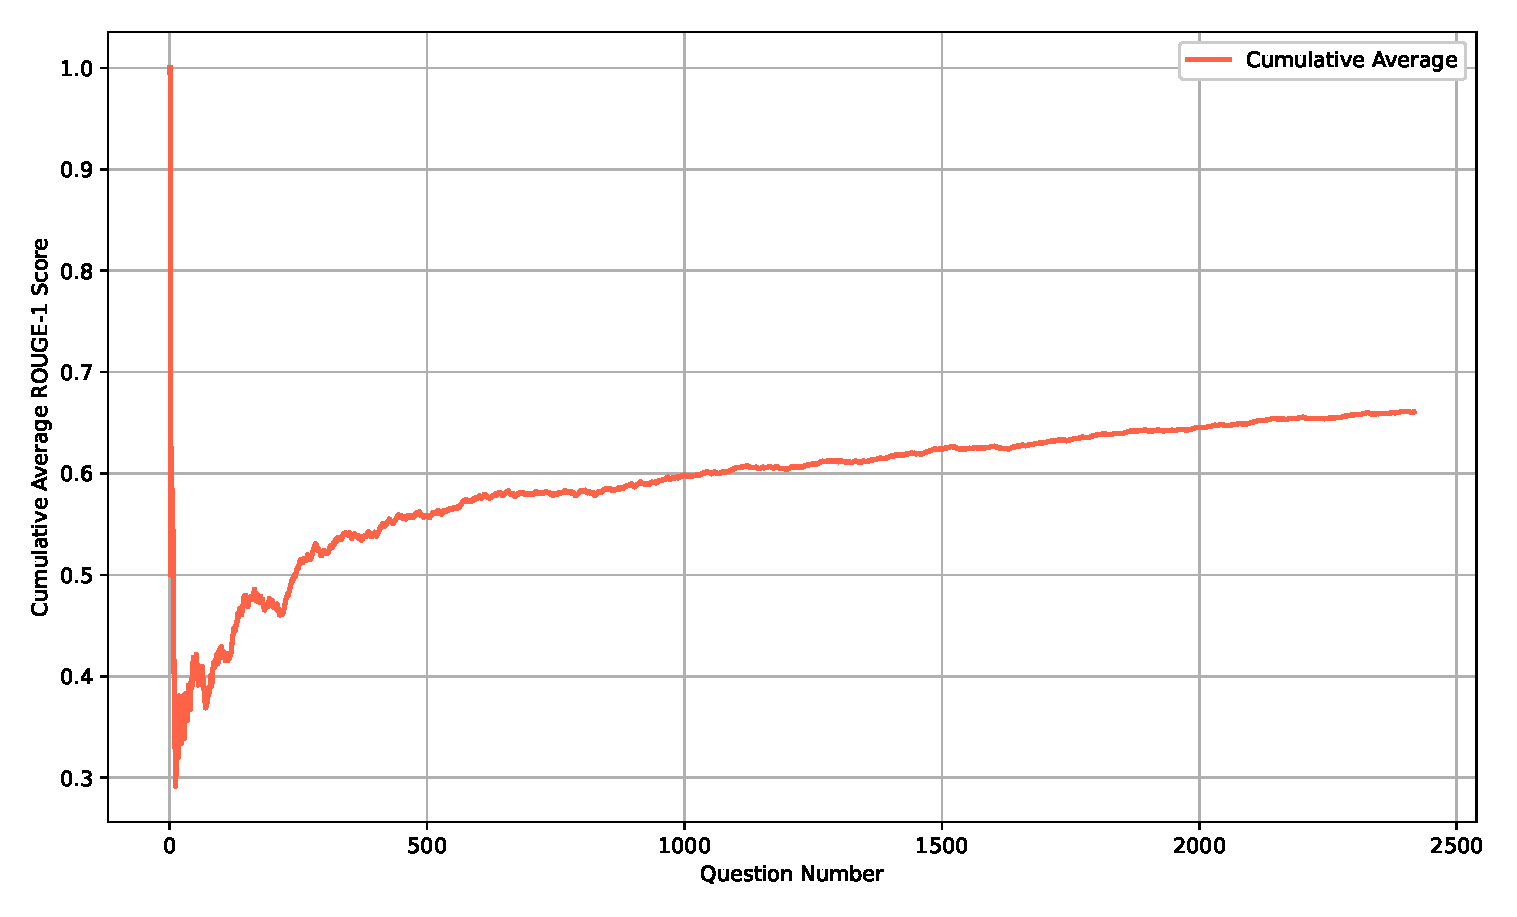
\includegraphics[width=.8\textwidth]{images/musique_cognitive_agent.eps}
    \caption{Cognitive QA Agent Learning on MuSiQue using $R_1$ cumulative average.}
    \label{fig:cog_agent_learn}
\end{figure}

\noindent To assess generalization, we further compare the QA Agent and the Cognitive QA Agent on samples not included in the original evaluation sets. For each dataset, we evaluate on 1000 additional questions. During this evaluation, the cognitive agent's memory is frozen, preventing the addition of new traces and forcing the model to rely exclusively on prior learning. Results, in Table \ref{tab:qa_results_agent_v2}, show no significant improvement compared to the baseline QA Agent, suggesting that while the cognitive architecture does not generalize well, it does maintain stable performance.

\begin{table}[ht]
    \centering
        \adjustbox{max width=1.1\textwidth}{
        \begin{tabular}{lcccccccccccccccc}
            \toprule
            & \multicolumn{4}{c}{\textbf{HotpotQA}} & \multicolumn{4}{c}{\textbf{2Wiki}} & \multicolumn{4}{c}{\textbf{MuSiQue}} & \multicolumn{4}{c}{\textbf{Average}} \\
            \cmidrule(lr){2-5} \cmidrule(lr){6-9} \cmidrule(lr){10-13} \cmidrule(lr){14-17}
            & EM & $R_1$ & $R_2$ & $L_1$ & EM & $R_1$ & $R_2$ & $L_1$ & EM & $R_1$ & $R_2$ & $L_1$ & EM & $R_1$ & $R_2$ & $L_1$ \\
            \midrule
            QA Agent & 70.8 & 78.4 & 44.7 & 81.0 & - & - & - & - & 46.2 & 53.6 & 31.0 & 54.0 & - & - & - & - \\
            Cognitive QA Agent & 70.4 & 78.0 & 44.1 & 80.0 & - & - & - & - & 45.7 & 53.5 & 30.6 & 54.0 & - & - & - & - \\
            \bottomrule
        \end{tabular}
        }
    \caption{\small Agents Question Answering performance on new questions.}
    \label{tab:qa_results_agent_v2}
\end{table}

